\documentclass{ximera}

%\usepackage{todonotes}

\newcommand{\todo}{}

\usepackage{esint} % for \oiint
\ifxake%%https://math.meta.stackexchange.com/questions/9973/how-do-you-render-a-closed-surface-double-integral
\renewcommand{\oiint}{{\large\bigcirc}\kern-1.56em\iint}
\fi


\graphicspath{
  {./}
  {ximeraTutorial/}
  {basicPhilosophy/}
  {functionsOfSeveralVariables/}
  {normalVectors/}
  {lagrangeMultipliers/}
  {vectorFields/}
  {greensTheorem/}
  {shapeOfThingsToCome/}
  {dotProducts/}
  {partialDerivativesAndTheGradientVector/}
  {../productAndQuotientRules/exercises/}
  {../normalVectors/exercisesParametricPlots/}
  {../continuityOfFunctionsOfSeveralVariables/exercises/}
  {../partialDerivativesAndTheGradientVector/exercises/}
  {../directionalDerivativeAndChainRule/exercises/}
  {../commonCoordinates/exercisesCylindricalCoordinates/}
  {../commonCoordinates/exercisesSphericalCoordinates/}
  {../greensTheorem/exercisesCurlAndLineIntegrals/}
  {../greensTheorem/exercisesDivergenceAndLineIntegrals/}
  {../shapeOfThingsToCome/exercisesDivergenceTheorem/}
  {../greensTheorem/}
  {../shapeOfThingsToCome/}
  {../separableDifferentialEquations/exercises/}
  {vectorFields/}
}

\newcommand{\mooculus}{\textsf{\textbf{MOOC}\textnormal{\textsf{ULUS}}}}

\usepackage{tkz-euclide}
\usepackage{tikz}
\usepackage{tikz-cd}
\usetikzlibrary{arrows}
\tikzset{>=stealth,commutative diagrams/.cd,
  arrow style=tikz,diagrams={>=stealth}} %% cool arrow head
\tikzset{shorten <>/.style={ shorten >=#1, shorten <=#1 } } %% allows shorter vectors

\usetikzlibrary{backgrounds} %% for boxes around graphs
\usetikzlibrary{shapes,positioning}  %% Clouds and stars
\usetikzlibrary{matrix} %% for matrix
\usepgfplotslibrary{polar} %% for polar plots
\usepgfplotslibrary{fillbetween} %% to shade area between curves in TikZ
%\usetkzobj{all}
\usepackage[makeroom]{cancel} %% for strike outs
%\usepackage{mathtools} %% for pretty underbrace % Breaks Ximera
%\usepackage{multicol}
\usepackage{pgffor} %% required for integral for loops



%% http://tex.stackexchange.com/questions/66490/drawing-a-tikz-arc-specifying-the-center
%% Draws beach ball
\tikzset{pics/carc/.style args={#1:#2:#3}{code={\draw[pic actions] (#1:#3) arc(#1:#2:#3);}}}



\usepackage{array}
\setlength{\extrarowheight}{+.1cm}
\newdimen\digitwidth
\settowidth\digitwidth{9}
\def\divrule#1#2{
\noalign{\moveright#1\digitwidth
\vbox{\hrule width#2\digitwidth}}}




% \newcommand{\RR}{\mathbb R}
% \newcommand{\R}{\mathbb R}
% \newcommand{\N}{\mathbb N}
% \newcommand{\Z}{\mathbb Z}

\newcommand{\sagemath}{\textsf{SageMath}}


%\renewcommand{\d}{\,d\!}
%\renewcommand{\d}{\mathop{}\!d}
%\newcommand{\dd}[2][]{\frac{\d #1}{\d #2}}
%\newcommand{\pp}[2][]{\frac{\partial #1}{\partial #2}}
% \renewcommand{\l}{\ell}
%\newcommand{\ddx}{\frac{d}{\d x}}

% \newcommand{\zeroOverZero}{\ensuremath{\boldsymbol{\tfrac{0}{0}}}}
%\newcommand{\inftyOverInfty}{\ensuremath{\boldsymbol{\tfrac{\infty}{\infty}}}}
%\newcommand{\zeroOverInfty}{\ensuremath{\boldsymbol{\tfrac{0}{\infty}}}}
%\newcommand{\zeroTimesInfty}{\ensuremath{\small\boldsymbol{0\cdot \infty}}}
%\newcommand{\inftyMinusInfty}{\ensuremath{\small\boldsymbol{\infty - \infty}}}
%\newcommand{\oneToInfty}{\ensuremath{\boldsymbol{1^\infty}}}
%\newcommand{\zeroToZero}{\ensuremath{\boldsymbol{0^0}}}
%\newcommand{\inftyToZero}{\ensuremath{\boldsymbol{\infty^0}}}



% \newcommand{\numOverZero}{\ensuremath{\boldsymbol{\tfrac{\#}{0}}}}
% \newcommand{\dfn}{\textbf}
% \newcommand{\unit}{\,\mathrm}
% \newcommand{\unit}{\mathop{}\!\mathrm}
% \newcommand{\eval}[1]{\bigg[ #1 \bigg]}
% \newcommand{\seq}[1]{\left( #1 \right)}
% \renewcommand{\epsilon}{\varepsilon}
% \renewcommand{\phi}{\varphi}


% \renewcommand{\iff}{\Leftrightarrow}

% \DeclareMathOperator{\arccot}{arccot}
% \DeclareMathOperator{\arcsec}{arcsec}
% \DeclareMathOperator{\arccsc}{arccsc}
% \DeclareMathOperator{\si}{Si}
% \DeclareMathOperator{\scal}{scal}
% \DeclareMathOperator{\sign}{sign}


%% \newcommand{\tightoverset}[2]{% for arrow vec
%%   \mathop{#2}\limits^{\vbox to -.5ex{\kern-0.75ex\hbox{$#1$}\vss}}}
% \newcommand{\arrowvec}[1]{{\overset{\rightharpoonup}{#1}}}
% \renewcommand{\vec}[1]{\arrowvec{\mathbf{#1}}}
% \renewcommand{\vec}[1]{{\overset{\boldsymbol{\rightharpoonup}}{\mathbf{#1}}}}

% \newcommand{\point}[1]{\left(#1\right)} %this allows \vector{ to be changed to \vector{ with a quick find and replace
% \newcommand{\pt}[1]{\mathbf{#1}} %this allows \vec{ to be changed to \vec{ with a quick find and replace
% \newcommand{\Lim}[2]{\lim_{\point{#1} \to \point{#2}}} %Bart, I changed this to point since I want to use it.  It runs through both of the exercise and exerciseE files in limits section, which is why it was in each document to start with.

% \DeclareMathOperator{\proj}{\mathbf{proj}}
% \newcommand{\veci}{{\boldsymbol{\hat{\imath}}}}
% \newcommand{\vecj}{{\boldsymbol{\hat{\jmath}}}}
% \newcommand{\veck}{{\boldsymbol{\hat{k}}}}
% \newcommand{\vecl}{\vec{\boldsymbol{\l}}}
% \newcommand{\uvec}[1]{\mathbf{\hat{#1}}}
% \newcommand{\utan}{\mathbf{\hat{t}}}
% \newcommand{\unormal}{\mathbf{\hat{n}}}
% \newcommand{\ubinormal}{\mathbf{\hat{b}}}

% \newcommand{\dotp}{\bullet}
% \newcommand{\cross}{\boldsymbol\times}
% \newcommand{\grad}{\boldsymbol\nabla}
% \newcommand{\divergence}{\grad\dotp}
% \newcommand{\curl}{\grad\cross}
%\DeclareMathOperator{\divergence}{divergence}
%\DeclareMathOperator{\curl}[1]{\grad\cross #1}
% \newcommand{\lto}{\mathop{\longrightarrow\,}\limits}

% \renewcommand{\bar}{\overline}

\colorlet{textColor}{black}
\colorlet{background}{white}
\colorlet{penColor}{blue!50!black} % Color of a curve in a plot
\colorlet{penColor2}{red!50!black}% Color of a curve in a plot
\colorlet{penColor3}{red!50!blue} % Color of a curve in a plot
\colorlet{penColor4}{green!50!black} % Color of a curve in a plot
\colorlet{penColor5}{orange!80!black} % Color of a curve in a plot
\colorlet{penColor6}{yellow!70!black} % Color of a curve in a plot
\colorlet{fill1}{penColor!20} % Color of fill in a plot
\colorlet{fill2}{penColor2!20} % Color of fill in a plot
\colorlet{fillp}{fill1} % Color of positive area
\colorlet{filln}{penColor2!20} % Color of negative area
\colorlet{fill3}{penColor3!20} % Fill
\colorlet{fill4}{penColor4!20} % Fill
\colorlet{fill5}{penColor5!20} % Fill
\colorlet{gridColor}{gray!50} % Color of grid in a plot

\newcommand{\surfaceColor}{violet}
\newcommand{\surfaceColorTwo}{redyellow}
\newcommand{\sliceColor}{greenyellow}




\pgfmathdeclarefunction{gauss}{2}{% gives gaussian
  \pgfmathparse{1/(#2*sqrt(2*pi))*exp(-((x-#1)^2)/(2*#2^2))}%
}


%%%%%%%%%%%%%
%% Vectors
%%%%%%%%%%%%%

%% Simple horiz vectors
\renewcommand{\vector}[1]{\left\langle #1\right\rangle}


%% %% Complex Horiz Vectors with angle brackets
%% \makeatletter
%% \renewcommand{\vector}[2][ , ]{\left\langle%
%%   \def\nextitem{\def\nextitem{#1}}%
%%   \@for \el:=#2\do{\nextitem\el}\right\rangle%
%% }
%% \makeatother

%% %% Vertical Vectors
%% \def\vector#1{\begin{bmatrix}\vecListA#1,,\end{bmatrix}}
%% \def\vecListA#1,{\if,#1,\else #1\cr \expandafter \vecListA \fi}

%%%%%%%%%%%%%
%% End of vectors
%%%%%%%%%%%%%

%\newcommand{\fullwidth}{}
%\newcommand{\normalwidth}{}



%% makes a snazzy t-chart for evaluating functions
%\newenvironment{tchart}{\rowcolors{2}{}{background!90!textColor}\array}{\endarray}

%%This is to help with formatting on future title pages.
\newenvironment{sectionOutcomes}{}{}



%% Flowchart stuff
%\tikzstyle{startstop} = [rectangle, rounded corners, minimum width=3cm, minimum height=1cm,text centered, draw=black]
%\tikzstyle{question} = [rectangle, minimum width=3cm, minimum height=1cm, text centered, draw=black]
%\tikzstyle{decision} = [trapezium, trapezium left angle=70, trapezium right angle=110, minimum width=3cm, minimum height=1cm, text centered, draw=black]
%\tikzstyle{question} = [rectangle, rounded corners, minimum width=3cm, minimum height=1cm,text centered, draw=black]
%\tikzstyle{process} = [rectangle, minimum width=3cm, minimum height=1cm, text centered, draw=black]
%\tikzstyle{decision} = [trapezium, trapezium left angle=70, trapezium right angle=110, minimum width=3cm, minimum height=1cm, text centered, draw=black]


\title{Tangent}

\begin{document}

\begin{abstract}
quotient
\end{abstract}
\maketitle







Tangent is the quotient of sine and cosine.

\[   \tan(\theta)  =  \frac{\sin(\theta)}{\cos(\theta)}  \]


\begin{itemize}
\item \textbf{zeros:} $\tan(\theta)$ has a zero everywhere that $\sin(\theta)$ has a zero:  all of the whole-$\pi$'s.
\item \textbf{singluaries:} $\tan(\theta)$ has a singularity everywhere that $\cos(\theta)$ has a zero:  all of the half-$\pi$'s.
\end{itemize}

This means intercepts at the whole-$\pi$'s and vertical asymptotes at the half-$\pi$'s.








\begin{image}
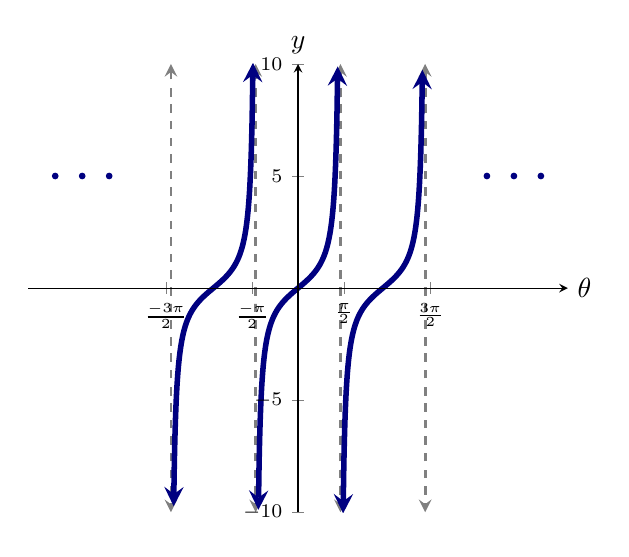
\begin{tikzpicture} 
  \begin{axis}[
            domain=-10:10, ymax=10, xmax=10, ymin=-10, xmin=-10,
            xtick={-4.9, -1.7, 1.7, 4.9}, 
            xticklabels={$\frac{-3\pi}{2}$, $\frac{-\pi}{2}$, $\frac{\pi}{2}$, $\frac{3\pi}{2}$},
            axis lines =center,  xlabel={$\theta$}, ylabel=$y$,
            ticklabel style={font=\scriptsize},
            every axis y label/.style={at=(current axis.above origin),anchor=south},
            every axis x label/.style={at=(current axis.right of origin),anchor=west},
            axis on top
          ]
          
            \addplot [line width=1, gray, dashed,samples=100,domain=(-10:10), <->] ({-4.71},{x});
            \addplot [line width=1, gray, dashed,samples=100,domain=(-10:10), <->] ({-1.57},{x});
            \addplot [line width=1, gray, dashed,samples=100,domain=(-10:10), <->] ({1.57},{x});
            \addplot [line width=1, gray, dashed,samples=100,domain=(-10:10), <->] ({4.71},{x});

            \addplot [line width=2, penColor, smooth,samples=100,domain=(-1.47:1.47), <->] {tan(deg(x))};
            \addplot [line width=2, penColor, smooth,samples=100,domain=(-4.61:-1.67), <->] {tan(deg(x))};
            \addplot [line width=2, penColor, smooth,samples=100,domain=(1.67:4.61), <->] {tan(deg(x))};

      \addplot[color=penColor,fill=penColor,only marks, mark size=1pt, mark=*] coordinates{(-9,5) (-8,5) (-7,5) (7,5) (8,5) (9,5)};


            

           

  \end{axis}
\end{tikzpicture}
\end{image}




\begin{itemize}
\item Tangent is always increasing.
\item Tangent has no maximums or minimum, since it is unbounded near the half-$\pi$'s.
\item The period for tangent is $\pi$.
\end{itemize}





\begin{example}




Analyze  $K(t) = -\tan(\frac{t}{2} + \pi)$



\begin{explanation}


The usual interval people look at tangent is $\left[  \frac{-\pi}{2}, \frac{\pi}{2} \right]$.  This interval has singularities on both ends, which signal vertical asymptotes on the graph. $\frac{-\pi}{2}$ and $\frac{\pi}{2}$ are what we need the inside of our function to equal.


\begin{align*}
\frac{t}{2} + \pi   & = \frac{-\pi}{2}   \\
\frac{t}{2}   & = \frac{-3\pi}{2}   \\
t             & = \answer{-3 \pi}
\end{align*}





\begin{align*}
\frac{t}{2} + \pi   & = \frac{\pi}{2}   \\
\frac{t}{2}   & = \frac{-\pi}{2}   \\
t             & = \answer{-\pi}
\end{align*}




The period is $\answer{2 \pi}$.  One of the arms of this tangent function sits on the interval $[ -3 \pi, - \pi ]$.



Then the $-1$ coefficient flips the graph upside-down.
















\begin{image}
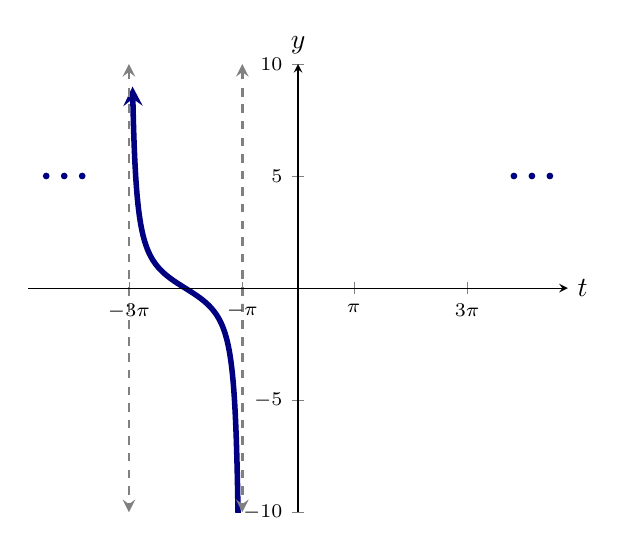
\begin{tikzpicture} 
  \begin{axis}[
            domain=-15:15, ymax=10, xmax=15, ymin=-10, xmin=-15,
            xtick={-9.4, -3.1, 3.1, 9.4}, 
            xticklabels={$-3\pi$, $-\pi$, $\pi$, $3\pi$},
            axis lines =center,  xlabel={$t$}, ylabel=$y$,
            ticklabel style={font=\scriptsize},
            every axis y label/.style={at=(current axis.above origin),anchor=south},
            every axis x label/.style={at=(current axis.right of origin),anchor=west},
            axis on top
          ]
          
            \addplot [line width=2, penColor, smooth,samples=100,domain=(-9.2:-3.25), <->] {-tan(deg(0.5*x+3.14))};
            %\addplot [line width=2, penColor, smooth,samples=100,domain=(-4.61:-1.67), <->] {tan(deg(x))};
            %\addplot [line width=2, penColor, smooth,samples=100,domain=(1.67:4.61), <->] {tan(deg(x))};

      \addplot[color=penColor,fill=penColor,only marks, mark size=1pt, mark=*] coordinates{(-14,5) (-13,5) (-12,5) (12,5) (13,5) (14,5)};


            \addplot [line width=1, gray, dashed,samples=100,domain=(-10:10), <->] ({-9.4},{x});
            \addplot [line width=1, gray, dashed,samples=100,domain=(-10:10), <->] ({-3.1},{x});
            %\addplot [line width=1, gray, dashed,samples=100,domain=(-10:10), <->] ({1.57},{x});
            %\addplot [line width=1, gray, dashed,samples=100,domain=(-10:10), <->] ({4.71},{x});

           

  \end{axis}
\end{tikzpicture}
\end{image}

There are no maximums or minimums.

$K(t)$ is always decreasing.

The zeros are $\{  2 k \pi \, | \, k \in \mathbb{Z}    \}$














\end{explanation}
\textbf{Notes:} \\


$\blacktriangleright$ Comparing $K(t)$ to $\tan(t)$, the inside has been multiplied by $\frac{1}{2}$.  This would indicate the perioid is doubled from $\pi$ to $2\pi$, which has happened.  

$\blacktriangleright$ Additionally, an $\pi$ hs been added to the inside.  This would indicate a horizontal shift left, which has happened.


\end{example}

































\subsection*{Geometry}


Sine and cosine come from measurements of the unit circle.  What about tangent?


Draw our usual right triangle for sine and cosine on the unit circle.  Draw a tangent line at the point on the circle.  Extend this line to the horizontal axis and use this to draw a second right triangle.  The two right triangles have an angle $\theta$, which means all three angles are equal, which means the triangles are similar.







\begin{image}
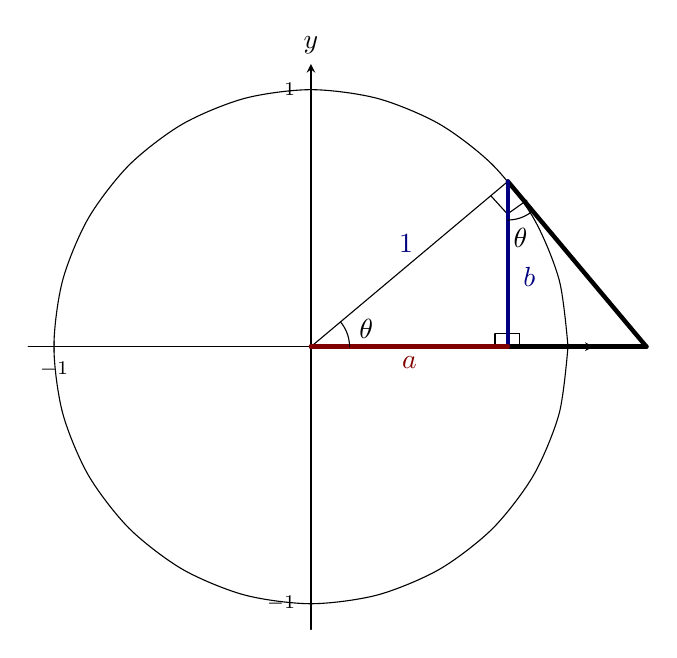
\begin{tikzpicture}[line cap=round]
  \begin{axis}[
            xmin=-1.1,xmax=1.1,ymin=-1.1,ymax=1.1,
            axis lines=center,
            width=4in,
            xtick={-1},
            ytick={-1,1},
            clip=false,
            unit vector ratio*=1 1 1,
            xlabel=$ $, ylabel=$y$,
            ticklabel style={font=\scriptsize},
            every axis y label/.style={at=(current axis.above origin),anchor=south},
            every axis x label/.style={at=(current axis.right of origin),anchor=west},
          ]        
          


          \draw [ultra thick] (axis cs:0,0) -- (axis cs:1.305,0);
          \draw [ultra thick] (axis cs:0.766,0.643) -- (axis cs:1.305,0);



          \draw [thin] (axis cs:0.716,0.05) -- (axis cs:0.766,0.05);
          \draw [thin] (axis cs:0.716,0) -- (axis cs:0.716,0.05);

          \draw [thin] (axis cs:0.766,0.05) -- (axis cs:0.812,0.05);
          \draw [thin] (axis cs:0.812,0) -- (axis cs:0.812,0.05);

          \draw [thin] (axis cs:0.7,0.587) -- (axis cs:0.77,0.51);
          \draw [thin] (axis cs:0.77,0.52) -- (axis cs:0.84,0.57);





          \addplot [smooth, domain=(0:360)] ({cos(x)},{sin(x)}); %% unit circle

          \addplot [textColor] plot coordinates {(0,0) (.766,.643)}; %% 40 degrees

          \addplot [ultra thick,penColor] plot coordinates {(.766,0) (.766,.643)}; %% 40 degrees
          \addplot [ultra thick,penColor2] plot coordinates {(0,0) (.766,0)}; %% 40 degrees
          
          %\addplot [ultra thick,penColor3] plot coordinates {(1,0) (1,.839)}; %% 40 degrees          

          \addplot [textColor,smooth, domain=(0:40)] ({.15*cos(x)},{.15*sin(x)});
          %\addplot [very thick,penColor] plot coordinates {(0,0) (.766,.643)}; %% sector
          %\addplot [very thick,penColor] plot coordinates {(0,0) (1,0)}; %% sector
          %\addplot [very thick, penColor, smooth, domain=(0:40)] ({cos(x)},{sin(x)}); %% sector
          \node at (axis cs:.15,.07) [anchor=west] {$\theta$};
          \node[penColor] at (axis cs:0.85,.27) {$b$};
          \node[penColor2] at (axis cs:.383,0) [anchor=north] {$a$};
          %\node[penColor3, rotate=-90] at (axis cs:1.06,.322) {$\tan(\theta)$};
           \node[penColor] at (axis cs:0.37,0.4) {$1$};


          \node at (axis cs:0.815, 0.5) [anchor=north] {$\theta$};
          \addplot [textColor,smooth, domain=(270:310)] ({0.15*cos(x)+0.766},{0.15*sin(x)+0.643});
          %\node[textColor] at (axis cs:1.1,0)[anchor=north] {$c$};
          %\node[textColor] at (axis cs:1.05,0.5)[anchor=north] {$h$};








        \end{axis}
\end{tikzpicture}
\end{image}
These two right triangles are similar.  There is also a third big right triangle.

















\begin{image}
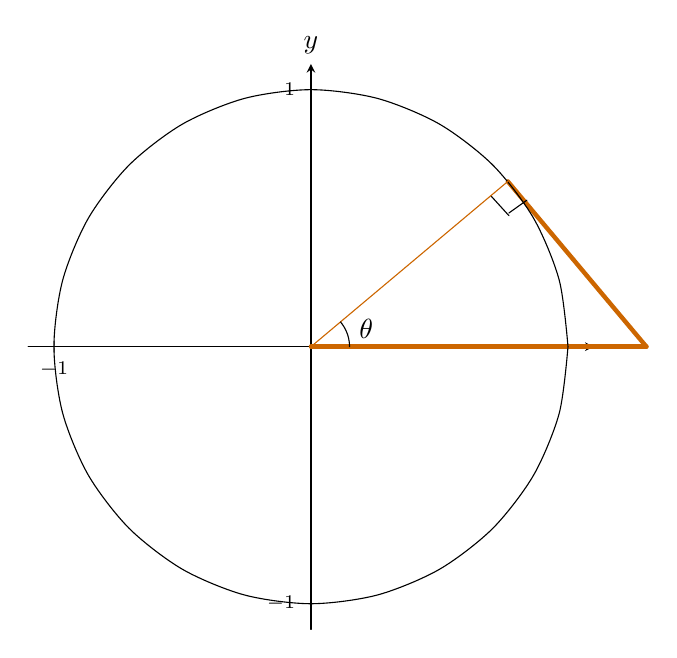
\begin{tikzpicture}[line cap=round]
  \begin{axis}[
            xmin=-1.1,xmax=1.1,ymin=-1.1,ymax=1.1,
            axis lines=center,
            width=4in,
            xtick={-1},
            ytick={-1,1},
            clip=false,
            unit vector ratio*=1 1 1,
            xlabel=$ $, ylabel=$y$,
            ticklabel style={font=\scriptsize},
            every axis y label/.style={at=(current axis.above origin),anchor=south},
            every axis x label/.style={at=(current axis.right of origin),anchor=west},
          ]        
          


          \draw [penColor5, ultra thick] (axis cs:0,0) -- (axis cs:1.305,0);
          \draw [penColor5, ultra thick] (axis cs:0.766,0.643) -- (axis cs:1.305,0);



          %\draw [thin] (axis cs:0.716,0.05) -- (axis cs:0.766,0.05);
          %\draw [thin] (axis cs:0.716,0) -- (axis cs:0.716,0.05);

          %\draw [thin] (axis cs:0.766,0.05) -- (axis cs:0.812,0.05);
          %\draw [thin] (axis cs:0.812,0) -- (axis cs:0.812,0.05);

          \draw [thin] (axis cs:0.7,0.587) -- (axis cs:0.77,0.51);
          \draw [thin] (axis cs:0.77,0.52) -- (axis cs:0.84,0.57);





          \addplot [smooth, domain=(0:360)] ({cos(x)},{sin(x)}); %% unit circle

          \addplot [penColor5] plot coordinates {(0,0) (.766,.643)}; %% 40 degrees

          %\addplot [ultra thick,penColor] plot coordinates {(.766,0) (.766,.643)}; %% 40 degrees
          %\addplot [ultra thick,penColor2] plot coordinates {(0,0) (.766,0)}; %% 40 degrees
          
          %\addplot [ultra thick,penColor3] plot coordinates {(1,0) (1,.839)}; %% 40 degrees          

          \addplot [textColor,smooth, domain=(0:40)] ({.15*cos(x)},{.15*sin(x)});
          %\addplot [very thick,penColor] plot coordinates {(0,0) (.766,.643)}; %% sector
          %\addplot [very thick,penColor] plot coordinates {(0,0) (1,0)}; %% sector
          %\addplot [very thick, penColor, smooth, domain=(0:40)] ({cos(x)},{sin(x)}); %% sector
          \node at (axis cs:.15,.07) [anchor=west] {$\theta$};
          %\node[penColor] at (axis cs:0.85,.27) {$b$};
          %\node[penColor2] at (axis cs:.383,0) [anchor=north] {$a$};
          %\node[penColor3, rotate=-90] at (axis cs:1.06,.322) {$\tan(\theta)$};
           %\node[penColor] at (axis cs:0.37,0.4) {$1$};


          %\node at (axis cs:0.815, 0.5) [anchor=north] {$\theta$};
          %\addplot [textColor,smooth, domain=(270:310)] ({0.15*cos(x)+0.766},{0.15*sin(x)+0.643});
          %\node[textColor] at (axis cs:1.1,0)[anchor=north] {$c$};
          %\node[textColor] at (axis cs:1.05,0.5)[anchor=north] {$h$};








        \end{axis}
\end{tikzpicture}
\end{image}






















Let's label some sides.


\begin{image}
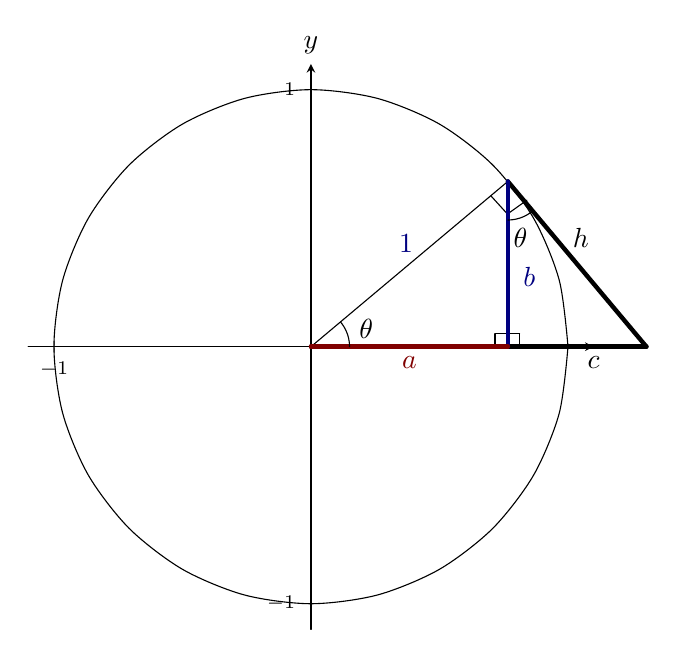
\begin{tikzpicture}[line cap=round]
  \begin{axis}[
            xmin=-1.1,xmax=1.1,ymin=-1.1,ymax=1.1,
            axis lines=center,
            width=4in,
            xtick={-1},
            ytick={-1,1},
            clip=false,
            unit vector ratio*=1 1 1,
            xlabel=$ $, ylabel=$y$,
            ticklabel style={font=\scriptsize},
            every axis y label/.style={at=(current axis.above origin),anchor=south},
            every axis x label/.style={at=(current axis.right of origin),anchor=west},
          ]        
          


          \draw [ultra thick] (axis cs:0,0) -- (axis cs:1.305,0);
          \draw [ultra thick] (axis cs:0.766,0.643) -- (axis cs:1.305,0);



          \draw [thin] (axis cs:0.716,0.05) -- (axis cs:0.766,0.05);
          \draw [thin] (axis cs:0.716,0) -- (axis cs:0.716,0.05);

          \draw [thin] (axis cs:0.766,0.05) -- (axis cs:0.812,0.05);
          \draw [thin] (axis cs:0.812,0) -- (axis cs:0.812,0.05);

          \draw [thin] (axis cs:0.7,0.587) -- (axis cs:0.77,0.51);
          \draw [thin] (axis cs:0.77,0.52) -- (axis cs:0.84,0.57);





          \addplot [smooth, domain=(0:360)] ({cos(x)},{sin(x)}); %% unit circle

          \addplot [textColor] plot coordinates {(0,0) (.766,.643)}; %% 40 degrees

          \addplot [ultra thick,penColor] plot coordinates {(.766,0) (.766,.643)}; %% 40 degrees
          \addplot [ultra thick,penColor2] plot coordinates {(0,0) (.766,0)}; %% 40 degrees
          
          %\addplot [ultra thick,penColor3] plot coordinates {(1,0) (1,.839)}; %% 40 degrees          

          \addplot [textColor,smooth, domain=(0:40)] ({.15*cos(x)},{.15*sin(x)});
          %\addplot [very thick,penColor] plot coordinates {(0,0) (.766,.643)}; %% sector
          %\addplot [very thick,penColor] plot coordinates {(0,0) (1,0)}; %% sector
          %\addplot [very thick, penColor, smooth, domain=(0:40)] ({cos(x)},{sin(x)}); %% sector
          \node at (axis cs:.15,.07) [anchor=west] {$\theta$};
          \node[penColor] at (axis cs:0.85,.27) {$b$};
          \node[penColor2] at (axis cs:.383,0) [anchor=north] {$a$};
          %\node[penColor3, rotate=-90] at (axis cs:1.06,.322) {$\tan(\theta)$};
           \node[penColor] at (axis cs:0.37,0.4) {$1$};


          \node at (axis cs:0.815, 0.5) [anchor=north] {$\theta$};
          \addplot [textColor,smooth, domain=(270:310)] ({0.15*cos(x)+0.766},{0.15*sin(x)+0.643});
          \node[textColor] at (axis cs:1.1,0)[anchor=north] {$c$};
          \node[textColor] at (axis cs:1.05,0.5)[anchor=north] {$h$};








        \end{axis}
\end{tikzpicture}
\end{image}




In the diagram above, we know that $a = \cos(\theta)$ and $b = \sin(\theta)$.

We also know the unit circle right triangles are both similar to the big right triangle, since they all include the angle $\theta$.

Since, they are similar, we know that 


\[    \frac{opp}{adj} = \frac{b}{a}  = \frac{\sin(\theta)}{\cos(\theta)}   = \frac{h}{1}          \]


\[         \tan(\theta) = h\]




$\tan(\theta)$ can be represented as the length of the tangent line segment, from the tangent point to the $x$-axis.









\begin{image}
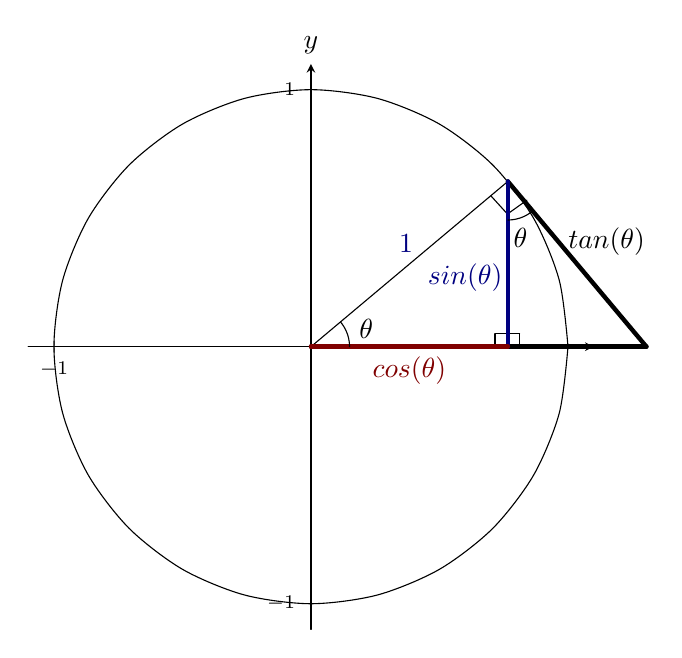
\begin{tikzpicture}[line cap=round]
  \begin{axis}[
            xmin=-1.1,xmax=1.1,ymin=-1.1,ymax=1.1,
            axis lines=center,
            width=4in,
            xtick={-1},
            ytick={-1,1},
            clip=false,
            unit vector ratio*=1 1 1,
            xlabel=$ $, ylabel=$y$,
            ticklabel style={font=\scriptsize},
            every axis y label/.style={at=(current axis.above origin),anchor=south},
            every axis x label/.style={at=(current axis.right of origin),anchor=west},
          ]        
          


          \draw [ultra thick] (axis cs:0,0) -- (axis cs:1.305,0);
          \draw [ultra thick] (axis cs:0.766,0.643) -- (axis cs:1.305,0);



          \draw [thin] (axis cs:0.716,0.05) -- (axis cs:0.766,0.05);
          \draw [thin] (axis cs:0.716,0) -- (axis cs:0.716,0.05);

          \draw [thin] (axis cs:0.766,0.05) -- (axis cs:0.812,0.05);
          \draw [thin] (axis cs:0.812,0) -- (axis cs:0.812,0.05);

          \draw [thin] (axis cs:0.7,0.587) -- (axis cs:0.77,0.51);
          \draw [thin] (axis cs:0.77,0.52) -- (axis cs:0.84,0.57);





          \addplot [smooth, domain=(0:360)] ({cos(x)},{sin(x)}); %% unit circle

          \addplot [textColor] plot coordinates {(0,0) (.766,.643)}; %% 40 degrees

          \addplot [ultra thick,penColor] plot coordinates {(.766,0) (.766,.643)}; %% 40 degrees
          \addplot [ultra thick,penColor2] plot coordinates {(0,0) (.766,0)}; %% 40 degrees
          
          %\addplot [ultra thick,penColor3] plot coordinates {(1,0) (1,.839)}; %% 40 degrees          

          \addplot [textColor,smooth, domain=(0:40)] ({.15*cos(x)},{.15*sin(x)});
          %\addplot [very thick,penColor] plot coordinates {(0,0) (.766,.643)}; %% sector
          %\addplot [very thick,penColor] plot coordinates {(0,0) (1,0)}; %% sector
          %\addplot [very thick, penColor, smooth, domain=(0:40)] ({cos(x)},{sin(x)}); %% sector
          \node at (axis cs:.15,.07) [anchor=west] {$\theta$};
          \node[penColor] at (axis cs:0.6,.27) {$sin(\theta)$};
          \node[penColor2] at (axis cs:.383,0) [anchor=north] {$cos(\theta)$};
          %\node[penColor3, rotate=-90] at (axis cs:1.06,.322) {$\tan(\theta)$};
           \node[penColor] at (axis cs:0.37,0.4) {$1$};


          \node at (axis cs:0.815, 0.5) [anchor=north] {$\theta$};
          \addplot [textColor,smooth, domain=(270:310)] ({0.15*cos(x)+0.766},{0.15*sin(x)+0.643});
          %\node[textColor] at (axis cs:1.1,0)[anchor=north] {$c$};
          \node[textColor] at (axis cs:1.15,0.5)[anchor=north] {$tan(\theta)$};








        \end{axis}
\end{tikzpicture}
\end{image}

Is this important?  Not really.  But, it is nice to collect all of our Trigonometric functions together on the unit circle.  It explains their names.










\begin{center}
\textbf{\textcolor{green!50!black}{ooooo-=-=-=-ooOoo-=-=-=-ooooo}} \\

more examples can be found by following this link\\ \link[More Examples of Trigonometric Functions]{https://ximera.osu.edu/csccmathematics/precalculus2/precalculus2/trigonometricFunctions/examples/exampleList}

\end{center}



\end{document}

